\section{Translation Theorem}\label{sec:translation}


\begin{theorem}\label{th:translate}
There is a polynomial time transformation, that maps a 
1-FPN(BC)-specification $\Gamma = (G(V,E), m)$ of the  graph $\Gamma^m$ 
to a strongly 1-level-restricted 
L-specification $\Gamma_1$ of a graph, 
such that the graphs represented by 
$\Gamma$ and $\Gamma_1$ are isomorphic and 
$size(\Gamma_1) = (size(\Gamma))^2$.
\end{theorem}

\noindent
{\bf Proof:} We discuss the transformation without boundary conditions first.
Given a {\sf 1-FPN}-specification  $\Gamma = G(V,E)$ of $G^m$ 
we construct a {\sf L}-specification $H_G = (H_1, \cdots H_n)$ as follows. 
The non-terminal $H_1$  consists of four copies of $G$ (i.e. $G^4$). 
They are connected in series as shown in Figure \ref{translation1.fig}(a), 

%\iffalse
%%%%
\begin{figure}[tbh]
\centering
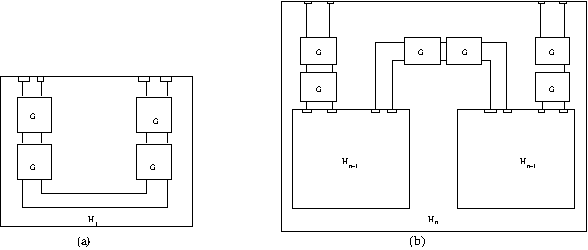
\includegraphics{translation1}
\caption{Construction of $H_i$, $1 \leq i \leq n$}
\label{translation1.fig}
\end{figure}
%%%%
%\fi




\noindent 
{\bf Non-terminal  $H_i$, $2 \leq i \leq n$:}
Asssume that the periodic graph is of the form $G^{2k}$.
The non-terminal $H_i$ consists of five components
$l_i$, $r_i$, $m_i$, $H_{i-1}$, $H_{i-1}$. 
Each of $l_i$, $r_i$ and  $m_i$ consists of at least 2 copies of $G$ 
($G^2$) attached in a manner as shown in the Figure \ref{translation1.fig}(b). 

Each $H_{i-1}$ recursively encodes $G^{p}$, 
We need to ensure that for each recursive
call $p$ is even, thus we need to adjust the sizes of 
the components $l_i$, $r_i$ and  $m_i$ accordingly.
The $H_{i-1}$'s 
are connected to the components $l_i$, $r_i$ and  $m_i$ as shown in 
Figure \ref{translation1.fig}(b). 
The condition that each $H_{i-1}$ have even number of copies of $G$ 
implies that the construction should satisfy the following constraints.
\[ |l_i|, ~ |r_i|, ~  |m_i| \geq 2 \]  
\[~~~ p = 2m \] 
\[2m + 2m + |l_i| + |r_i| +  |m_i| = 2k \]  


The first constraint is needed so that the resulting specification is 
1-level-restricted. The second equation says that $p$ is even. This is needed 
so that each of the smaller indexed non-terminals  
can be defined recursively. 
The third equation says that the 
total number of copies of $G$ is no more than $2k$, which is the size of the
graph we want to encode. It is clear that the sizes of $l_i$, 
$r_i$ and $m_i$ can be chosen  so that the above equations can be satisfied.
The process can be
carried out recursively to obtain the required specification $H$
in polynomial time.

Observe that a similar transformation can be carried out if we start
with a {\sf 1-FPN(BC)} specified graph $G$. 
In this case the graphs which specify the boundary conditions
are included in the highest non-terminal.\QED

Using similar ideas we can transform {\sf 1-FPN}-specified formulas into
isomorphic {\sf L}-specified formulas. Thus we have the following corollary.


\begin{corollary}\label{cor:translate}
There is a polynomial time transformation that maps a 
1-FPN(BC)-specification $\Gamma = (U, C(i, i+1), m)$ of the formula $\Gamma^m$ 
to a strongly 1-level-restricted 
L-specification $\Gamma_1$ such that
that the formulas represented by $\Gamma$ and $\Gamma_1$ are isomorphic and
$size(\Gamma_1)= O((size(\Gamma))^2)$ 
\end{corollary}
